\chapter{Implémentation du Simulateur et Modélisation d'une Colonie d'Abeilles}
\label{ChapitrePropSMA}

	Nous allons désormais aborder dans ce chapitre l'implémentation du modèle que nous venons de décrire, appliqué au cas qui nous intéresse ici : la colonie d'abeilles. Pour cette première version, nos abeilles virtuelles auront pour objectif de correctement se répartir le travail entre deux tâches principales : "Nourrir le couvain" et "Butiner". Nous allons commencer par discuter de notre simulateur et de son architecture logicielle, puis du modèle physiologique de l'abeille adulte et du couvain, tiré de la biologie présentée au Chapitre \ref{ChapitreContexte} de Contexte, mais simplifié au maximum. Nous verrons ensuite comment nous avons intégré le modèle de répartition des tâches décrit dans le chapitre précédent. Nous finirons par discuter de la calibration de ce système complexe, au plus proche de la biologie, tout en prenant en compte les différentes hypothèses et simplifications de notre modèle.
	
	\section{Description du Simulateur}
		\subsection{Architecture Logicielle}
			Pour réaliser ce simulateur, nous avions en tête quelques points clés : l'idée est de produire un simulateur propre, qui serait simple d'entretien et facile à améliorer et complexifier par la suite, au-delà des travaux de thèse présentés ici. Un compromis entre confort d'écriture et performances qu'offre Java, ainsi que notre bonne maitrise du langage nous a poussé à l'utiliser. Pour nous aider à mettre en place ces notions de propreté du code, nous avons utilisé des Interfaces Java, permettant de découpler de grandes parties du programme, facilitant l'implémentation de modifications. Nous avons pensé l'architecture en composants indépendants échangeant le moins d'informations possibles. Nous allons désormais décrire les principaux composants de cette architecture, la Figure \ref{ArchiLogicielle} résume le tout graphiquement.
			
			\begin{figure}
			\centering
			\includegraphics[width=\textwidth]{./Pictures/Figures/ArchiLogicielle.png}
			\caption{Diagramme UML de classe esquissant l'architecture logicielle du simulateur.}
			\label{ArchiLogicielle}
			\end{figure}
			
			Le simulateur est pensé en couches d'abstraction successives. Au plus haut niveau, nous trouvons le lanceur, la classe \textit{BeekeeperLauncher}, le célèbre "\textit{main}", le point d'entrée du programme, qui se charge des simulations. Il présente deux modes :
	\begin{itemize}
		\item Interactions : ce mode permet de lancer une simulation et est prévu pour recevoir les interactions de l'utilisateur (via le réseau) pour altérer le comportement de la simulation, et renvoie une importante quantité de données par ce même réseau.
		\item Barrage de Simulations : mode permettant de lancer un grand nombre de simulations à la suite, sans interactions possibles. Ce mode sert principalement pour calibrer certains paramètres et effectuer des expérimentations.
	\end{itemize}				
			
			 La Figure \ref{ArchiStart} illustre la séquence d'appels au lancement du programme. Dans le mode "Interactions", le lanceur prépare le composant réseau \textit{NetworkManager} qui servira à envoyer et recevoir les informations de l'application interactive, composant qui n'est pas instancié dans le mode "Barrage de Simulations". Sur la figure, cette étape est notée "1b", signifiant qu'elle n'est réalisée que dans le cas du mode "Interaction". Le lanceur instancie ensuite le \textit{MainController} (1 sur la figure), le contrôleur principal, et lui partage le composant réseau (1b) si besoin. Le \textit{MainController} se charge de gérer une simulation. Désormais nous trouvons deux comportements différents pour les modes : en "Barrage de Simulations", les simulations s'enchaînent à pleine vitesse, souvent en variant quelques paramètres. En mode "Interactions", lorsque la simulation est arrêtée, soit le programme s'arrête soit une autre est relancée avec les mêmes paramètres, selon ce qui a été décidé par l'utilisateur.
			 
			\begin{figure}
			\centering
			\includegraphics[width=\textwidth]{./Pictures/Figures/ArchiStart.png}
			\caption{Séquencement de l'initialisation d'une simulation.}{1- Le lanceur \textit{BeekeeperLauncher} instancie et initialise le \textit{MainController} qui se chargera d'une simulation. 1b- Dans le cas où le lanceur est dans le mode Interactions, il instancie un \textit{NetworkManager} et en donne la référence au MainController (Lors d'un changement de simulation, le \textit{MainController} est remplacé mais le \textit{NetworkManager} reste le même). 2- Le \textit{MainController} se charge désormais d'instancier un \textit{CombManager} avec les bons paramètres. 3- Le \textit{CombManager} commence par initialiser les \textit{Cadres}, il instancie en réalité des faces de cadres qu'il va associer par deux pour former les cadres de la simulation. 4- Une fois créés, les \textit{Cadres} sont alors peuplés par le \textit{CombManager} avec des \textit{Agents}. 5- Ensuite, des \textit{StimuliManager} sont instanciés par le \textit{CombManager} et associés à des faces de cadres.}
			\label{ArchiStart}
			\end{figure}
			
			Le \textit{MainController} se charge d'instancier correctement les différents composants d'une simulation et du bon déroulement de l'ensemble. Il compte les pas de temps, ce qui lui permet d'envoyer un signal aux agents, via un autre composant, leur ordonnant de vivre un pas de temps (pour éviter les biais, les agents sont activés dans un ordre aléatoire). Via une interface Java, il offre un grand nombre de services haut niveau à différents composants, notamment au \textit{CombManager}, le manager des cadres, qu'il instancie avec les bons paramètres (étape 2 de la Figure \ref{ArchiStart}). Le \textit{CombManager} se charge d'instancier le bon nombre de faces de cadres (3) modélisés par la classe "\textit{Comb}", qui seront associées par deux pour former les cadres. Il instancie ensuite les agents initiaux (4) et les répartit sur ces cadres, via un autre composant, l'\textit{AgentFactory}, qui simplifie et centralise la création d'agents.
			
			Visible sur la Figure \ref{ArchiLogicielle}, chaque face de cadre possède une liste de cellules, représentées par la classe \textit{Cell}, qui elles-mêmes possèdent quelques attributs : leur numéro et leur position x et y sur le cadre ($numéro = y * largeur + x$), ainsi qu'une place "visite" pour un agent qui serait au-dessus de la cellule, et une place "contenu", pour un agent à l'intérieur de la cellule ou de la nourriture, ou même rien, pour une cellule vide. Chaque face de cadre possède une liste contenant tous les agents que contiennent ces cellules. Cette liste agit comme un raccourci, et permet de ne pas avoir à interroger toutes les cellules à chaque fois que nous voulons accéder aux agents. Le \textit{CombManager} possède aussi une liste d'agents, ceux qui n'appartiennent à aucun cadre : la liste de tous les agents à l'extérieur de la ruche, les butineuses.
			
			Le \textit{CombManager} est aussi responsable de la création, mise à jour, et bonne association des \textit{StimuliManager}, les managers de propagation des différents stimulus dans l'environnement. Cette instanciation est notée "5" sur la figure \ref{ArchiStart}. Les cadres sont placés les uns à côtés dans autres, les faces se faisant face partagent le même \textit{StimuliManager}. 
			
			La Figure \ref{Env} schématise l'environnement de nos agents, les cadres et faces de cadres. Nous y voyons huit cadres, dont les faces ont été labellisées de "A" à "P". Un cadre est composé de deux faces "dos à dos", par exemple le premier cadre est composé des faces "A" et "B". Les agents présents sur la face de cadre "A" sont indépendants de ceux sur la face "B". En revanche, les agents présents sur des faces opposées, par exemple les faces "B" et "C" interagissent entre eux, et peuvent aller d'une de ces deux faces à l'autre lors d'un déplacement classique. Les stimulus émis sur une face sont ressentis sur la face opposée, ainsi chaque \textit{StimuliManager} gère deux faces de cadres en même temps.
			\begin{figure}
			\centering
			\includegraphics[width=\textwidth]{./Pictures/Figures/Env.png}
			\caption[Schéma vu de côté de l'organisation des cadres et faces de cadres.]{Schéma de l'organisation des cadres et faces de cadres. La face de cadre "D" est détaillée sur la droite (seules quelques cellules hors échelle sont représentées pour des raisons de lisibilités). Les faces de cadres "N" et "O" sont dites "opposées", elles se font faces. Les faces "E" et "F" sont "dos à dos", elles forment le troisième cadre.}
			\label{Env}
			\end{figure}
			
			%POUR LES INTERACTIONS AVEC LE MODELE
			%Lorsque les cadres sont déplacés, de nouveaux \textit{StimuliManager} temporaires doivent être créés pendant le déplacement, puis lorsqu'ils sont reposés dans la ruche, le \textit{CombManager} se charge de refaire les bonnes associations, et combinaisons avec les temporaires.
			
			Un \textit{StimuliManager} est une grille 2D de la même taille qu'un cadre, dont chaque case possède plusieurs valeurs réelles, représentant les intensités des différents stimulus présents sur les faces de cadres opposées (principalement des phéromones, mais aussi des vibrations). Ainsi, une case de cette grille représente deux cellules "face à face". La mise à jour de cette grille utilise une méthode de "\textit{double buffering}" : la grille est lue et une deuxième est remplie avec les valeurs mises à jour. Une fois la lecture terminée, la deuxième grille prend la place de la première. La propagation se fait à chaque pas de temps pour chaque stimulus et, afin de gagner du temps, l'évaporation se fait en même temps que le calcul de la propagation. Pour propager les stimulus, nous utilisons une fonction proche d'un flou en traitement d'image. Chaque pixel devient une moyenne pondérée de lui-même et de tous ses voisins. Chaque case voit son intensité devenir la moyenne pondérée de sa propre intensité et de celles de ses voisines, en suivant cette équation :
			
			\begin{figure}
			\centering
			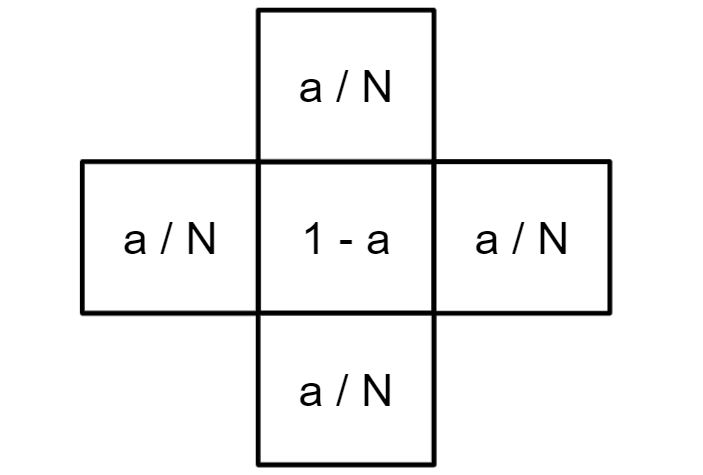
\includegraphics[width=0.4\textwidth]{./Pictures/Figures/flou.JPG}
			\caption[Filtre utilisé pour connaitre la nouvelle valeur de l'intensité du stimulus évalué.]{Filtre utilisé pour connaitre la nouvelle valeur de l'intensité du stimulus évalué. Avec $a$ la volatilité du stimulus évalué, et $N$ le nombre de voisins, ici $N=4$. Chaque pixel prend alors comme valeur la combinaison linéaire de sa valeur et de celles de ses voisins avec ce filtre pour coefficient.}
			\label{flou}
			\end{figure}
			
			\begin{equation}
			V0_{t+1} = p * ((1-a) * V0_t + \sum_{n=1}^{N} Vn_t * \frac{a}{N})
			\end{equation}
			
			avec $V0_t$ la case évaluée à l'instant $t$, $Vn$ ses voisines et $N$ le nombre total de voisines. Nous utilisons aussi $a$ et $p$ deux paramètres de stimulus : la propagation dans l'espace $a$ (volatilité) et dans le temps $p$ (évaporation/amortissement). Ces paramètres nous permettent d'obtenir des comportements variés partageant les mêmes mécanismes. La Figure \ref{flou} illustre cette équation sous la forme d'un filtre. Les valeurs d'évaporations sont alors utilisées sous la forme "par pas de temps". Pour mieux les contrôler, nous utilisons l'équation suivante pour les exprimer en demi-vie (durée après laquelle le stimulus aura perdu la moitié de son intensité), notion plus courante en biologie, puis les convertir en valeurs "par pas de temps" utilisables par l'algorithme :
			
			\begin{equation}
			k = \exp(\frac{-ln(2) * C}{\lambda})
			\end{equation}
			
			avec $\lambda$ la demi-vie en seconde, $C$ le coefficient appliqué pour convertir des secondes en pas de temps, et $k$ le coefficient à appliquer à chaque pas de temps pour obtenir une demi-vie de $\lambda$.
			
			\subsection{Architecture des Agents}
			Les mêmes objectifs en tête, lisibilité et facilité d'ajouts, nos agents ont été pensés en niveaux d'abstraction successifs. Au plus haut niveau nous trouvons la classe abstraite \textit{Agent}, qui regroupe l'âge, la position, l'énergie, la faim, une fonction abstraite \textit{live} (vivre), ainsi que des méthodes de déplacement simples, comme le mouvement aléatoire. La partie droite de la Figure \ref{ArchiLogicielle} présente l'architecture des agents. Nous définissons la classe \textit{EmitterAgent}, ou Agent Émetteur, qui hérite d'\textit{Agent} et ajoute les interactions avec un \textit{StimuliManager}, permettant d'émettre et de ressentir des stimulus dans l'environnement. Enfin, héritant d'\textit{EmitterAgent}, nous trouvons la classe \textit{WorkingAgent}, ou Agent Travailleur, qui implémente \textit{live}, avec l'algorithme de sélection de tâches présenté Chapitre \ref{ChapitrePropDecision} et détaillé section \ref{subsectionImplemTasks}. La fonction \textit{live} se déroule en quatre étapes. Nous vérifions tout d'abord si l'agent est toujours en vie, ensuite nous mettons à jour ses perceptions. L'algorithme de sélection et exécution des tâches est alors appliqué, puis une fonction abstraite est appelée, fonction permettant de faire avancer le métabolisme de l'agent, et qui est implémentée différemment par chaque implémentation de \textit{WorkingAgent}. Nous avons pour l'instant 3 classes implémentant cette dernière, les classes d'abeille adulte \textit{AdultBee}, de couvain \textit{BroodBee}, et de reine \textit{QueenBee}. Chacune de ces implémentations ajoute différentes tâches à sa liste de tâches (que nous allons décrire Section \ref{sectionModelColonie}), et implémente la fonction d'avancer du métabolisme.
			
			Ainsi, dans les plus hautes couches d'abstraction, les différents composants ont des références \textit{Agent}, ce qui améliore la modularité du programme, facilitant l'ajout de nouvelles implémentations de \textit{WorkingAgent} à l'avenir. 
			
			\subsection{Pas de temps et Multi-Thread}
			Afin d'accélérer nos simulations pour itérer plus confortablement dessus, nous avons mis en place un système de parallélisation, aussi appelé \textit{multi-thread}. Les agents présents sur une face de cadre peuvent interagir entre eux et avec les agents situés sur la face de cadre opposée (voir Figure \ref{Env}). Ils n'interagissent pas avec les autres agents présents sur d'autres cadres, de la même manière que les stimulus ne se propagent pas à ces autres cadres : cela nous permet de considérer chaque couple de faces de cadre opposées comme des ensembles indépendants. Les butineuses n'étant sur aucun cadre, elles représentent un nouvel ensemble indépendant. Afin de s'assurer que ces ensembles vivent en concurrence, nous avons créé la classe \textit{WorkDispatcher}, qui s'occupe de gérer un groupe d'\textit{ExecutorThread}, de leur répartir la charge, d'en créer de nouveaux si nécessaire et de surveiller le moment où tous ont terminé leur travail. À chaque pas de temps, sur signal du \textit{MainController}, le \textit{CombManager} récupère et combine si nécessaire les différents groupes d'agents à faire vivre ensemble. Pour reprendre la Figure \ref{Env}, le \textit{CombManager} assemble les agents de la face "B" avec ceux de "C", ceux de "D" avec ceux de "E" etc. Les agents de "A", de "P", et les agents extérieurs sont laissés seuls. Il envoie alors ces ensembles au \textit{WorkDispatcher} qui redirige les listes sur des \textit{ExecutorThread} disponibles. Chaque \textit{ExecutorThread} va alors appeler la fonction \textit{live} de chacun des agents de sa liste. La Figure \ref{ArchiThread} illustre ces échanges.
			
			\begin{figure}
			\centering
			\includegraphics[width=\textwidth]{./Pictures/Figures/ArchiThread.png}
			\caption{Séquencement de la partie d'un pas de temps concernant les agents.}{1- Le \textit{MainController} envoie le signal au \textit{CombManager} de faire vivre les agents d'un pas de temps. 2- Celui-ci va alors récupérer les listes d'agents présents sur les cadres ainsi que celle des agents en cours de butinage. 3- Il réarrange ensuite ces listes en rassemblant les agents ne pouvant pas vivre en concurrence, puis envoie ces listes aux \textit{WorkDispatcher}. 4- Ce-dernier va ensuite envoyer ces listes à des \textit{ExecutorThread} et en instancier de nouveaux s'il le faut. Ils vont alors, chacun en concurrence, parcourir leur liste d'agents et les faire vivre chacun leur tour. 5- Enfin, lorsque le \textit{WorkDispatcher} détecte que tous les threads ont terminé de faire vivre leurs agents, il le signal au \textit{CombManager} qui rend alors la main au \textit{MainController}.}
			\label{ArchiThread}
			\end{figure}
			
			Pour le cas particulier des agents en cours de butinage ré-entrant ou quittant l'environnement (la ruche), deux listes synchronisées spéciales ont été ajoutées au niveau du \textit{CombManager}. Une liste contenant tous les agents qui sont sortis de la ruche sur ce pas de temps, et une liste contenant ceux qui sont rentrés. Les agents en extérieur et les agents sur les cadres ne vivant pas sur les même \textit{threads}, un agent rentrant ne peut pas être ajouté directement au cadre. Ce n'est qu'après avoir fait vivre tout le monde, que le \textit{CombManager} se charge de faire les transferts, déplaçant les agents sortants vers la liste des agents extérieurs, et les agents entrants vers un cadre libre aléatoire.
			
			Ensuite, lorsque tous les agents ont vécu, et que les déplacements entre cadres ont été réalisés, le \textit{CombManager} rend la main au \textit{MainController} qui se charge alors de terminer le pas de temps. Dans le mode "Barrage de Simulations", le pas de temps suivant est exécuté juste après, de la même manière que le précédent. En revanche, en mode "Interactions", le \textit{MainController} va effectuer une courte pause. Cette pause lui permet de s'assurer que tous ses pas de temps ont la même durée, et que cette durée correspond au temps réel. Nous avons choisi qu'un pas de temps représente une seconde, le contrôleur effectue donc une pause d'une seconde, en en déduisant le temps de calcul du pas de temps courant. Tous nos pas de temps sont ainsi séparés d'exactement une seconde. Dans le cas théorique où le calcul d'un pas de temps serait plus long que le temps qu'il est censé représenter, le \textit{MainController} enchainerait directement avec le pas de temps suivant, se rapprochant ainsi autant que possible de notre temps réel voulu.
			
			Ce temps réel est nécessaire pour permettre à l'utilisateur d'interagir avec les agents sans créer de biais dans la simulation. Lorsque l'utilisateur décide d'accélérer le temps pour observer l'état futur de la colonie, le \textit{MainController} cesse de faire ces pauses entre les pas de temps, comme dans le mode "Barrage de Simulations", ce qui permet de grandement accélérer les calculs, mais interdisant toutes interactions (simuler 80 jours ne prend que quelques minutes).
			
			\subsection{Architecture des Tâches}
			\label{subsectionImplemTasks}
			Nos tâches sont décrites en subsomptions hiérarchiques dans le modèle, nous les avons donc implémentées de la sorte dans le simulateur. Comme décrit par la Figure \ref{ArchiTask}, au sommet de la hiérarchie nous trouvons la classe \textit{Tâche}, associant un seuil, un nom de tâche, différents paramètres et une activité racine. Une \textit{Tâche} est une classe abstraite : toute classe que nous voudrons instancier devra implémenter la fonction qui permet de calculer son score, et peupler l'Activité racine d'Actions et/ou d'Activités.
			
			Visible sur la Figure \ref{ArchiTask}, la classe \textit{TaskNode}, ou Nœud de Tâche, est une interface très simple contenant deux fonctions : \textit{search} (recherche) et \textit{check} (vérifier). Elles nous permettent de mettre en place le fonctionnement de subsomption. La fonction \textit{check} représente la condition de chacun des blocs de notre subsomption, condition booléenne que chaque Nœud devra implémenter. Ensuite, la fonction \textit{search}, la principale, diffère selon les nœuds. La classe \textit{TaskNode} est implémentée par deux classes, \textit{Activité} et \textit{Action}, respectant notre modèle vu plus tôt. La fonction \textit{search} renvoie toujours une \textit{Action}, et permet d'interroger récursivement toute la subsomption hiérarchique. La fonction \textit{search} de la classe Action renvoie l'instance d'\textit{Action} sur laquelle elle est appelée. En revanche, une \textit{Activité} possède une liste de \textit{TaskNode}, permettant la mise en place de la subsomption hiérarchique. Dans la fonction \textit{search}, l'\textit{Activité} va interroger une par une (dans l'ordre de priorité de la subsomption) la fonction \textit{check} de tous ses nœuds. Si l'un d'eux valide son \textit{check}, l'\textit{Activité} appelle alors le \textit{search} du nœud validé, continuant la recherche en profondeur si appelé sur une Activité, ou mettant ainsi fin à la recherche lorsque appelé sur une Action.
			
			\begin{figure}
			\centering
			\includegraphics[width=0.8\textwidth]{./Pictures/Figures/ArchiTask.png}
			\caption{Diagramme de classe de l'architecture logicielle de Tâche.}
			\label{ArchiTask}
			\end{figure}
			
			Ainsi, pour qu'un agent puisse récupérer l'\textit{Action} à effectuer de sa \textit{Tâche} sélectionnée, il lui suffit d'appeler \textit{search} sur l'\textit{Activité} racine de la \textit{Tâche}. Récursivement, la recherche va descendre dans la subsomption dans les blocs aux conditions validées. Dès qu'une \textit{Action} est trouvée, sa fonction \textit{search} la renvoie et elle est remontée dans toutes les fonctions \textit{search} appelées précédemment, jusqu'à ressortir au niveau du tout premier \textit{search} que nous avons appelé sur l'\textit{Activité} racine de la \textit{Tâche}. L'\textit{Action} est prête à être exécutée par l'agent.
			
			
			Une fois tous les agents mis à jour, si le contrôleur principal a demandé d'enregistrer le tour, alors une nouvelle mécanique s'enclenche. Le manageur des cadres récupère à nouveau la liste de tous les agents, et leur demande de décrire en une ligne leur état : numéro d'identifiant, tâche, énergie, Hormone Juvénile (HJ) et Oléate d'Éthyle (OE). À cette ligne est ajouté au début le numéro du pas de temps transmis par le contrôleur principal. Toutes ces lignes sont alors envoyées au \textit{Logger}, qui les transfère sur un autre \textit{thread} afin d'être écrites dans un fichier, permettant une trace de la simulation, pour utilisations ultérieures en analyse de résultats.
			
			\paragraph{}			
			Pour résumer, lors d'un pas de temps, le contrôleur principal demande au manager des cadres de faire vivre tous les agents. Ce dernier parcourt alors toutes ses faces de cadres et récupère tous leurs agents, afin de les envoyer au gestionnaire de threads pour une exécution parallèle. Une fois tous les agents mis à jour, les agents entrant et sortant de la ruche sont transférés. Le contrôleur principal peut alors décider d'enregistrer ou non ce pas de temps. Ensuite, il termine ce pas de temps. S'il est en mode "Interaction" il va effectuer une pause afin de respecter le temps réel. Ensuite, un nouveau pas de temps est simulé.
			
	\section{Modélisation de la Colonie d'Abeilles}
	\label{sectionModelColonie}
		\subsection{Modélisation des Agents "Abeille Adulte"}
		
		Dans le \textit{Chapitre \ref{ChapitreContexte}} nous avons décrit l'importance des phéromones dans la physiologie, et la répartition des tâches (via l'âge du premier butinage). Les bouquets de phéromones émis par la reine, le couvain et les abeilles adultes influent les physiologies et comportements des adultes. Nous avons simplifié ces nombreuses interactions dans cette première version du modèle, afin de se concentrer sur la répartition des nourrices et des butineuses. Dans notre colonie virtuelle, les ouvrières adultes (qui sont désormais des agents) tendent toutes à aller butiner rapidement, grâce à l'Hormone Juvénile (HJ) qu'elles sécrètent, mais sont retenues "nourrices" par l'Oléate d'Éthyle (OE) émise par le couvain et les butineuses, qui "détruit" une part de leur HJ. L'OE n'est normalement qu'une composante des bouquets de phéromones, mais nous considérons ici qu'elle en représente la totalité. L'Ocimène présentée dans le Chapitre  \ref{ChapitreContexte} de Contexte qui a un effet inverse (elle pousse au butinage) n'est pas modélisée. De plus, les phéromones de la reine ne sont pas non plus modélisées, nous n'attendons donc pas de comportement de "cour royale", et n'avons pas modélisé les réponses des ouvrières à une colonie sans reine (ce qu'elles détectent normalement par l'absence des phéromones de reine).
		
			
			\begin{figure}
			\centering
			\includegraphics[width=\textwidth]{Pictures/Figures/ImplemDynamics.png}
			\caption[Notre modélisation de la physiologie de l'abeille adulte.]{Modélisation simplifiée des effets physiologiques responsables de l'auto-organisation.}
			\label{HJEODynamics}
			\end{figure}
		
		La rétroaction HJ-OE permet de réguler le nombre de nourrices et de butineuses au sein de la colonie : lorsqu'il y a beaucoup de couvain, très peu d'adultes vont partir butiner, car le couvain va injecter de grande quantité d'OE dans les agents de la colonie, et certaines butineuses peuvent même redevenir des nourrices. Lorsque les butineuses meurent de vieillesse, elles freinent moins le développement des nourrices, et certaines pourront partir butiner. Ces différentes interactions ont été synthétisées Figure \ref{HJEODynamics}. Dans les colonies réelles, les butineuses échangent très régulièrement des phéromones avec les receveuses, qui sont chargées de délester les butineuses de leur cargaison pour aller les stocker dans un endroit adapté dans la ruche. Nous posons une hypothèse ici, qui est que les receveuses sont un vecteur majeur de l'effet rajeunissant des butineuses sur les nourrices. Or, comme nous ne simulons pas de tâches de receveuses dans cette version du modèle, nous nous attendons à ne presque pas observer ce mécanisme.
		
		L'Hormone Juvénile (HJ) représente directement la physiologie de nos agents abeilles adultes, ce que nous appelons l'âge physiologique en référence au polyéthisme d'âge que nous observons dans les colonies réelles. Un agent avec très peu d'HJ ($HJ < 0.5$), sera capable de nourrir le couvain mais incapable de butiner. À l'inverse, un agent avec un fort taux d'HJ ($HJ > 0.5$), sera capable de butiner mais incapable de nourrir le couvain (ces mécanismes sont décrits le Chapitre \ref{ChapitreContexte} de Contexte). \textbf{Nous parlons donc de nourrices lorsque nous considérons les agents physiologiquement jeunes, et de butineuses pour les agents physiologiquement âgés}. Nous avons ajouté un paramètre à nos agents, leur développement ovarien qui est toujours nul sauf pour la reine pour qui il vaut 1. Cette variable n'est pas utilisée dans cette version de l'implémentation, mais permettra de simuler les ouvrières pondeuses que nous retrouvons dans la réalité, lorsque les phéromones de la reine ne parviennent plus à certaines ouvrières en périphérie de la colonie et que ces dernières commencent à pondre.
		
		Les abeilles d'hiver peuvent vivre jusqu'à une année entière \cite{mattila_timing_2001}, mais les butineuses meurent en une trentaine de jours, avec en moyenne les dix derniers jours passés à butiner. Les biologistes pensent que le vol est une activité très épuisante, et qu'il est possible qu'il réduise fortement l'espérance de vie des butineuses. Nous avons donc implémenté ce mécanisme pour les morts de vieillesses de nos agents. Ils meurent en une année, mais subissent une pénalité lorsqu'ils butinent. Ainsi, un agent qui butine voit son âge effectif (celui qui est utilisé pour déterminer la mort de vieillesse) augmenter trente fois plus vite qu'un agent à l'intérieur de la colonie.
		
		Nos agents sont placés sur le cadre et savent que la sortie de la ruche s'effectue par le bas (et savent aller vers le bas). Le travail de butinage est laissé très simple, le fourragement ne faisant pas partie de nos priorités ici. En effet, ce mécanisme passionnant fait déjà l'objet de grandes quantités de recherches, et nous nous concentrons ici sur l'intérieur de la ruche. À l'avenir, une simulation plus poussée des mécanismes de fourragement, sélection des sources de nectar, recrutement, etc. pourraient être ajoutés au modèle (nous avons travaillé sur un modèle de butinage \cite{riviere_toward_2018,riviere_modemulti-agent_2021} en parallèle de ces travaux, qui pourra tout à fait être intégré par la suite). Pour l'instant, les butineuses sortent de la ruche, attendent simplement pendant un nombre donné de pas de temps puis rentrent à nouveau dans la ruche, sur un cadre aléatoire possédant une case disponible au niveau de sa ligne la plus basse. La durée de ce butinage est, pour l'instant, systématiquement la même pour tous les agents. Elle correspond à une valeur moyenne des temps de butinage observés pour des butineuses réelles.
		
		
		\subsection{Modélisation du Couvain}
		
			Nous avons modélisé les trois étapes majeures de la vie du couvain : œuf, larve et nymphe. Seule la larve requiert de la nourriture, les deux autres étapes n'ont pas besoin de nourrice pour se dérouler correctement. La nymphe n'émet aucune phéromone, la cellule étant fermée et l'OE que nous avons modélisée étant transmise par contact. Un agent larve émet de l'OE en permanence, nous avons aussi fait le choix de faire émettre ces phéromones par les agents œufs. Plusieurs aspects ont motivé ce choix, que nous n'avons pas pu confirmer ou infirmer en biologie : l'œuf est pondu par la reine qui émet des phéromones très puissantes, elle en transmet donc surement à l'œuf pendant la ponte. De plus, n'ayant pas simulé les receveuses, le mécanisme de rajeunissement des nourrices par les butineuses est minoré, l'œuf permet donc de compenser légèrement ce biais. L'œuf ayant une durée de vie très courte, seulement 3 jours sur les 21 totaux avant l'émergence, il est tout à fait possible que cette émission n'ait quasiment aucun effet.
			
			Les phéromones émisent par les agents du couvain le long de leur vie vont altérer la physiologie des agents adultes. Elles sont échangées lorsqu'un agent adulte passe sur la case d'un agent couvain, et en plus grande quantité lorsqu'un agent effectuant la tâche de nourrice vient déposer de la nourriture à un agent larve, du fait du contact prolongé avec celle-ci.
		
	\subsection{Tâches et Auto-Organisation}
		Le but de notre simulation est de retrouver un équilibre dans le partage des tâches entre ces deux tâches clés : "Butiner" et "Nourrir le Couvain". Ces deux tâches ne présentent pas de stimulus déclencheur direct comme nous avons pu en discuter dans le chapitre précédent. Nous avons donc recours à une motivation source pour ces deux tâches, que nous plaçons initialement arbitrairement à $0.5$. Cette motivation source est abaissée à 0 lorsque l'abeille n'est pas physiologiquement apte à réaliser la tâche, ou, pour le butinage, si l'agent n'a pas suffisamment d'énergie pour survivre aux vols aller et retour. 
		
		Ensuite, nous utilisons l'HJ de chaque agent pour ajuster le seuil de chacune de ces deux tâches. Moins une abeille a d'HJ, plus elle aura de chance de sélectionner la tâche de nourrice, et plus une abeille aura d'HJ, plus elle aura de chance de sélectionner la tâche de butineuse (La description des modèles à seuils se trouve Section \ref{subsectionRTM}). Les seuils ont été ajustés pour empêcher les scores des tâches de dépasser $0.8$ : l'intervalle $[0.8 ; 1]$ est réservé aux tâches prioritaires, que nous allons maintenant décrire. En effet, si nos agents doivent se répartir deux tâches principales, ce ne sont pas les seules, nous avons ajouté des tâches d'entretiens : se reposer, donner à manger, demander à manger. Ces tâches ne sont pas motivées, elles possèdent des stimulus déclencheurs : la faim et l'énergie. La tâche de repos est prioritaire, son score est donc autorisé à dépasser $0.8$. 
		
		En effet, si l'énergie d'un agent devient négative, il meurt\footnote{Dans cette version du modèle nous avons fait le choix de ne représenter la nourriture qu'au plus simple. Ainsi, la mort par sous alimentation ne fait pas partie de cette version. L'importance des butineuses en est donc fortement réduite : même si 100\% de la colonie s'occupe du couvain, il y aura toujours suffisamment de nourriture. Ajouter la nourriture, détailler ses mécanismes de distribution et introduire son mécanisme de collecte est une des perspectives privilégiées pour la suite.}. Le couvain possède aussi trois tâches très simple, une pour chacune de ses étapes de développement. Ces différentes tâches altèrent seulement leurs émissions de phéromones (en effet, le seul rôle du couvain est de se nourrir). La reine possède une tâche lui permettant de pondre. La Table \ref{tableTasks} présente un récapitulatif de toutes les tâches implémentées.
		
		\begin{table}
        \centering
        \caption{Les différentes tâches que nos agents peuvent exécuter.}
        \begin{tabular}{|l|l|}
            \hline
            Nom de tâche & Calcul du score\\
            \hline
            \hline
            \multicolumn{2}{|l|}{Tâches d'entretien}\\
            \hline
            Se reposer & 1-Energie [0;1]\\
            Demander à manger & Faim [0;0.8] \\
            Donner à manger & Stimulus de demande détecté [0;0.8] \\
            Déplacement aléatoire & 0.2 (tâche par défaut) \\
            \hline
            \hline
            \multicolumn{2}{|l|}{Tâches Principales (et motivées)}\\
            \hline
            Butiner & 0 si $HJ<0.5$, sinon Sigmoïde seuil : 1-HJ déplacé dans [0.3;1] \\
            Nourrir le couvain & 0 si $HJ>0.5$, sinon Sigmoïde seuil : HJ déplacé dans [0.3;1] \\
            \hline
            \hline
            \multicolumn{2}{|l|}{Tâches du couvain et de la reine}\\
            \hline
            Tâche d'oeuf & 1 si âge d'oeuf, 0 sinon (le couvain n'a pas besoin de repos)\\
            Tâche de larve & 1 si âge de larve, 0 sinon\\
            Tâche de nymphe & 1 si âge de nymphe, 0 sinon \\
            Pondre & 0.8 si développement ovarien, 0 sinon\\
            \hline
            
        \end{tabular}
        \label{tableTasks}
    \end{table}
    
	\section{Calibration des Phéromones}
	
	La répartition des tâches au sein de la colonie, en particulier le nourrissage et le butinage, dépendent majoritairement de mécanismes d'hormones et de phéromones. Comme nous l'avons vu plus tôt, nous nous intéressons ici aux interactions entre l'Hormone Juvénile (HJ) et l'Oléate d'Éthyle (OE), comme décrit Figure \ref{HJEODynamics}.
	
	Paramétrer cette dynamique a été un processus complexe : notre grande simplification du modèle, et surtout des différentes phéromones nous détache, pour cette partie, de la réalité biologique. Nous avons donc émis des hypothèses, fixé des paramètres arbitrairement, dans le but de retrouver d'autres "macro-paramètres" émergents. Les deux points clés de cette paramétrisation sont 1. la quantité relative d'OE émise par rapport à l'HJ, et 2. la force des effets de l'HJ et de l'OE. De plus, la paramétrisation s'articule autour de deux points d'équilibre. Le premier, l'équilibre en OE ($OE_{Eq}$), qui représente le moment où un agent a suffisamment d'OE pour parfaitement compenser son vieillissement, et donc son émission d'HJ. L'autre point d'équilibre, cette fois en HJ ($HJ_{Eq}$), représente le moment où un agent sécrète la bonne quantité d'HJ pour parfaitement compenser l'évaporation d'OE, et donc maintenir le niveau de cette dernière.
	
	\subsection{Hypothèses et décisions arbitraires}
	Pour l'instant, les quantités absolues des différentes substances ne sont en rien liées à la réalité, nous avons donc pu choisir arbitrairement les quantités et points d'équilibres. Il sera peut-être intéressant par la suite de les faire correspondre aux quantités relevées sur les abeilles réelles, mais cette approche ne présentait pas d'intérêt, par rapports à la difficulté apportée, pour cette première version. Nous avons donc décidé de fixer la quantité d'HJ dans $[0;1]$, et $HJ_{Eq} = 0.8$. De son côté, la quantité d'OE est simplement comprise dans $[0;\infty[$, et avec $OE_{Eq} = 1$. 
	
	Ainsi, un agent abeille adulte avec un taux d'HJ supérieur à $HJ_{Eq}$ va émettre plus d'OE qu'il ne s'en évapore sur lui, permettant à l'OE de s'accumuler, le faisant potentiellement rajeunir. Un agent avec un taux d'OE inférieur à $OE_{Eq}$ va éliminer moins d'HJ qu'il n'en émet, et va donc vieillir.
	
	\paragraph{}
	Nous faisons ici l'hypothèse que la réduction d'HJ par l'OE se fait seulement avec une fonction prenant en compte la quantité d'OE. De même pour l'émission d'OE en fonction de la quantité d'HJ qui ne se fait que via une fonction dépendante de la quantité d'HJ de l'agent concerné. Nous posons aussi que ces fonctions ont la forme $x^n$, avec $n$ un paramètre fixé expérimentalement (que nous décrirons plus tard) et $x$ la différence entre le taux courant et la valeur d'équilibre donnée plus tôt.
	
	Les deux effets énoncés précédemment sont imbriqués dans une boucle de rétroaction. Les quantités absolues de ces éléments ne sont donc pas pertinentes, en revanche, les écarts entre ces deux produits provoquent la dynamique que nous recherchons. Nous avons ainsi décidé, pour simplifier le paramétrage, d'en fixer un et de chercher le deuxième. Nous avons donc fixé l'émission d'OE en fonction de l'HJ avec la fonction linéaire :
	
	\begin{equation}
		OE_{em} = (HJ - HJ_{Eq}) * OE_{Evap}
	\label{eoEM}
	\end{equation}

avec $OE_{Evap}$ la quantité d'OE qui s'évapore lorsque l'on considère une quantité d'OE égale à $OE_{Eq}$. Nous retrouvons donc la fonction sous la forme $s=x^n$ décrite plus tôt, avec $n = 1$ et $x$ l'écart d'HJ à l'équilibre facteur de $OE_{Evap}$.
	
	
	\subsection{Intensités des effets}	
	Après avoir fixé ces paramètres, nous devons nous atteler à trouver la bonne combinaison d'intensité des effets des substances, ainsi que la quantité à laquelle on veut les émettre. Pour l'HJ, il suffit de prendre le point de transition, nous avons choisi 0.5, et de le diviser par la quantité de pas de temps minimum qu'il faut pour l'atteindre. Nous pourrions décider de la majorer légèrement afin de prendre en compte l'effet de l'OE, ralentissant très légèrement le vieillissement en faible quantité. Ce ralentissement est cependant très faible pour un agent isolé, ainsi nous n'avons pas gardé l'option de la majoration.
	
	Nous avons ainsi la quantité d'HJ émise par chaque agent à chaque pas de temps, que nous appellerons désormais $HJ_{Incr}$. L'OE présente sur chaque agent viendra éliminer une partie de son HJ, combattant ainsi indirectement cet $HJ_{Incr}$, dont nous pouvons désormais nous servir comme référence. Nous voulons qu'à $OE_{Eq}$, la réduction d'HJ $HJ_{red}$ soit égale à $HJ_{Incr}$, pour compenser parfaitement le vieillissement de l'agent. Nous pouvons donc écrire :
	
	\begin{equation}
		 HJ_{red} = (OE - OE_{Eq})^n * HJ_{Incr}
	\label{hjRED}
	\end{equation}
	
	avec $n$ un coefficient dont nous allons nous servir pour modeler l'intensité de l'effet de réduction d'HJ. Avec $n=1$ (Figure \ref{eoLinear}), notre fonction est linéaire, nous nous servirons de cette fonction comme base de comparaison. Lorsque $n>1$, on obtient une fonction quadratique (Figure \ref{eoSquared}). L'effet rajeunissant de l'OE est diminué sous $OE_{Eq}$ et amplifié au-delà. Nous obtenons donc un vieillissement ainsi qu'un rajeunissement plus rapide. L'effet de l'OE est amplifié lorsque $n$ augmente. Enfin, avec $n < 1$, on obtient une fonction racine (Figure \ref{eoSqrt}). De la même manière, avec une racine, l'intensité des effets de l'OE est réduite.
	
	Pour illustrer, nous pouvons aussi imaginer que l'abeille vieillit naturellement rapidement. Mais, cet état d'équilibre est altéré par l'OE, nous pouvons donc visualiser ceci comme l'abeille étant attachée par un ressort à ce point d'équilibre. La rigidité de ce ressort peut alors être interprétée comme la puissance de l'OE, proportionnelle à n. Plus n est grand, plus l'abeille sera tirée rapidement vers ce point d'équilibre.
	
	Nous n'avons pas trouvé de moyen de fixer mathématiquement $n$, ni dans la littérature, ni même après mûres réflexions : il a donc été trouvé expérimentalement, nous y reviendrons dans la partie suivante, concernant la calibration.
	
	\begin{figure}
	\centering
	
	\begin{subfigure}{\textwidth}
	\centering
	\includegraphics[width=.9\textwidth]{Pictures/Figures/EOEffectsLINEAR.png}
	\caption{Réduction d'HJ \textbf{linéaire} (exposant $= 1$) par l'abeille en fonction de la quantité d'OE qu'elle possède. Lorsque $OE = OE_{Eq}$, la réduction compense parfaitement le vieillissement naturel de l'agent : $HJ_{Red} = HJ_{Incr}$.}
	\label{eoLinear}
	\end{subfigure}
	
	\begin{subfigure}{\textwidth}
	\centering
	\includegraphics[width=.9\textwidth]{Pictures/Figures/EOEffectsSquared.png}
	\caption{Lorsque la fonction de réduction est \textbf{quadratique} (exposant $> 1$) plutôt que linéaire (Fig \ref{eoLinear}), on observe à gauche que l'OE a moins de puissance sous $OE_{Eq}$, et beaucoup plus au-dessus. À droite, on voit donc que le vieillissement (lorsque $OE < OE_{Eq}$) ainsi que le rajeunissement ($OE > OE_{Eq}$) sont plus intenses.}
	\label{eoSquared}
	\end{subfigure}
	
	\begin{subfigure}{\textwidth}
	\centering
	\includegraphics[width=.9\textwidth]{Pictures/Figures/EOEffectsSQRT.png}
	\caption{Lorsque la fonction de réduction est \textbf{une racine} (exposant $< 1$) plutôt que linéaire (Fig \ref{eoLinear}), on observe à gauche que l'OE a plus de puissance sous $OE_{Eq}$, et beaucoup moins au-delà. À droite, on voit donc que le vieillissement ($OE < OE_{Eq}$) ainsi que le rajeunissement ($OE > OE_{Eq}$) sont plus doux.}
	\label{eoSqrt}	
	\end{subfigure}
	
	\caption[Différents degrés de fonctions pour ajuster l'intensité des effets de l'oléate d'éthyle sur les abeilles adultes.]{Différents degrés de fonctions pour ajuster l'intensité des effets de l'oléate d'éthyle sur les abeilles adultes. Pour toutes les figures, à gauche les flèches indiquent la force de réduction de l'OE, à droite elles indiquent la vitesse de vieillissement (en rouge lorsque l'agent vieillit, en bleu lorsqu'il rajeunit).}	
	\label{eoAll}
	\end{figure}
	
	
	
	\subsection{Quantités Émises par les Agents Larves}
	\label{subsesctionPHLarves}
	Un autre point clé de ce modèle est la capacité des agents larves à influer directement sur la physionomie des adultes, en contraignant certain à rester physiologiquement jeunes. Il faut donc que ces larves en émettent la bonne quantité : trop peu et il n'y aura pas assez de nourrices pour s'occuper du couvain, trop et il n'y aura plus assez de butineuses à la récolte de nourriture.
	
	La quantité d'OE émise par chaque larve est donc importante, car elle est censée permettre à l'abeille de rester jeune, et même de rajeunir. Nous avons donc commencé par placer cette émission à $OE_{Evap}$ (voir équation \ref{eoEM}). De plus, les contacts étant assez brefs, l'émission d'OE des larves doit permettre à une nourrice sollicitée de rester jeune malgré quelques temps de trajets. Ce dernier point porte une incertitude liée à l'émergence de ce comportement : la répartition des larves sur le cadre, les temps de trajets des nourrices entre les larves qui accepteront de la nourriture, l'aléatoire dans le trajet même que va choisir la nourrice, etc. Nous avons donc décidé de placer l'émission des larves à $k * OE_{Evap}$, avec k un coefficient que nous allons trouver expérimentalement, qui sera forcément supérieur à 1. En effet, nous savons qu'en dessous les larves n'auront pas le pouvoir d'empêcher les nourrices de vieillir et de partir butiner par la suite. La question est donc de savoir à quel point il doit être supérieur à 1.
	
	\subsection{Objectifs de calibration}
	\label{subsectionObjectifCalibration}
	Nous saurons que le coefficient $k$ de l'émission d'OE des larves est juste lorsque, peu importe la quantité de larves, la proportion de nourrices par rapport aux butineuses sera globalement constante. Avec une émission trop importante, augmenter le nombre de larves va drastiquement augmenter le ratio de nourrices. Par exemple, lors d'un essai nous obtenions 50\% de nourrices dans la population d'adultes pour 500 larves, mais presque 100\% de nourrices pour 1000 larves. À l'inverse, lorsque trop peu de nourrices sont captées par le couvain, ce coefficient doit être augmenté.
	
	Ensuite, il arrive qu'il faille diminuer la quantité d'OE émise par les larves alors qu'elle est déjà trop faible pour un petit nombre de larves (ou vice versa). C'est ici le signal que l'intensité des effets de l'OE sur les adultes est à ajuster en variant l'exposant de l'équation donnant $HJ_{Red}$ (Eq \ref{hjRED}). Ainsi, lorsque 500 larves maintiennent un ratio nourrices/butineuses correct mais faible, mais que 1000 retiennent trop de nourrices, c'est que l'OE a trop d'effet, il faut alors abaisser l'exposant de $HJ_{Red}$. 
	
	Nous avons gardé un exposant entier lorsqu'il est supérieur à 1, et de la forme $1/x$ (avec $x$ entier) pour un exposant inférieur à 1.
	
	
	Ce mécanisme par échange de phéromones est à la base de ce que nous cherchons à démontrer ici, et est profondément émergent, car dépendant des interactions entre tous nos agents, ce qui explique notre recours ici à un paramétrage expérimental. La méthodologie et les résultats de la calibration seront présentés et discutés dans le chapitre suivant.
			
	\section*{Synthèse}
		Dans ce chapitre nous avons discuté de l'architecture logicielle du simulateur, moteur de notre première version du modèle de la colonie. Nos agents à l'intérieur de la colonie doivent se répartir deux tâches automatiquement, "Nourrir les larves" et "Butiner". Plusieurs couches d'abstraction nous offrent une grande modularité dans le développement, et l'utilisation de plusieurs \textit{thread} d'exécution permet d'accélérer la simulation, nous permettant d'itérer plus confortablement sur le modèle. Nous avons ensuite décrit l'implémentation concrète du modèle de sélection et d'interruption de tâche, à partir de ce que nous avons pu construire au chapitre précédent : les seuils pour la physiologie de l'agent, modéliser les tâches en Activité ainsi qu'en Action, parfois démotivante, etc. Nous avons aussi décrit l'implémentation du modèle physiologique simplifié de l'abeille adulte, ses glandes, hormones, phéromones et leurs influences mutuelles ainsi que sur le comportement de nos agents. Après calibration de certains paramètres émergents difficiles à précalculer ou à estimer, nos agents devraient être capables de se répartir le travail sans contrôle central, et de manière dynamique, en s'adaptant aux changements d'environnement et de populations. 
		
		Dans le chapitre suivant nous allons pouvoir nous intéresser à cette auto-organisation : comment la mesurer, est-elle satisfaisante ? Nous parlerons aussi de calibration expérimentale, amenée par le caractère émergent de beaucoup de paramètres à retrouver nous venant d'observations de colonies réelles.
		